\documentclass[titlepage, a4paper]{article}
%\usepackage{euler}
\usepackage{graphicx, amssymb, amsmath, textcomp, booktabs}
\usepackage[libertine,vvarbb]{newtxmath}
\usepackage[scr=rsfso]{mathalfa}
% \usepackage[lining,semibold,type1]{libertine} % a bit lighter than Times--no osf in math
\usepackage[T1]{fontenc} % best for Western European languages
\usepackage{minted}
\usepackage{listings, color, setspace, titlesec, fancyhdr, mdframed, multicol}
\usepackage{ucharclasses}
\usepackage{xunicode, xltxtra}
\usepackage[inner=1.35cm, outer=0.9cm, top=1.7cm, bottom=0.0cm]{geometry}
\usepackage{pdfpages}
\usepackage{tocloft}
\usepackage{nameref}
\usepackage{verbatim}
\usepackage{relsize}
\usepackage{fontspec}
\usepackage[colorlinks, linkcolor = black]{hyperref}
\usepackage[table]{xcolor}
\usepackage{tabularx}
\usepackage{graphicx}
\usepackage{float}
% configure fonts
% if not using CJK
% \newfontfamily\substitutefont{SimSun}[Scale=0.8,BoldFont=SimHei]
% \setTransitionsForChinese{\begingroup\substitutefont}{\endgroup}
\usepackage{xeCJK}
\setCJKmainfont{Microsoft YaHei}[Scale=0.8]
\setCJKmonofont{SimHei}[Scale=0.8]
\setCJKsansfont{KaiTi}[Scale=0.8]

\setmainfont{Cambria}[Scale=0.925]
\setmonofont{Consolas}[Scale=0.775]
%\setsansfont{Gill Sans Medium}

\XeTeXlinebreaklocale "zh"
\XeTeXlinebreakskip = 0pt plus 1pt

\setlength{\parindent}{0em}\setlength{\parskip}{1pt}
\setlength\itemsep{1pt}

\makeatletter
\renewcommand{\paragraph}{%
	\@startsection{paragraph}{4}%
	{\z@}{1pt \@plus 1pt \@minus 1pt}{-1em}%
	{\normalfont\normalsize\bfseries}%
}
\makeatother


%configure the top corners
\pagestyle{fancy}
\setlength{\headsep}{0.1cm}

\chead{Acm template}
\rhead{Page \thepage}
\lhead{black\_trees}

%configure space between the two columns
\setlength{\columnsep}{13pt}

%configure minted to display codes
%\definecolor{Gray}{rgb}{0.9,0.9,0.9}

%remove leading numbers in table of contents
%\setcounter{secnumdepth}{0}	

%configure section style of table of content
\renewcommand\cftsecfont{\Large}

%configure section style
\titleformat{\section}
{\huge}			% The style of the section title
{\thesection.}				% a prefix
{4pt}						% How much space exists between the prefix and the title
{}					% How the section is represented
% \titleformat{\section}{\huge}{}{0pt}{}
\titlespacing{\section}{0pt}{0pt}{0pt}
\titlespacing{\subsection}{0pt}{0pt}{0pt}
\titlespacing{\subsubsection}{0pt}{0pt}{0pt}

%enable section to start new page automatically
%\let\stdsection\section
%\renewcommand\section{\penalty-100\vfilneg\stdsection}

%\renewcommand\theFancyVerbLine{\arabic{FancyVerbLine}}
\renewcommand{\theFancyVerbLine}{\sffamily \textcolor[rgb]{0.5,0.5,0.5}{\scriptsize {\arabic{FancyVerbLine}}}}

\setminted[cpp]{
	style=xcode,
	mathescape,
	linenos,
	autogobble,
	baselinestretch=0.8,
	tabsize=3,
	fontsize=\normalsize,
	%bgcolor=Gray,
	frame=single,
	framesep=1mm,
	framerule=0.3pt,
	numbersep=1mm,
	breaklines=true,
	breaksymbolsepleft=2pt,
	%breaksymbolleft=\raisebox{0.8ex}{ \small\reflectbox{\carriagereturn}}, %not moe!
	%breaksymbolright=\small\carriagereturn,
	breakbytoken=false,
	showtabs=true,
	tab={\relscale{0.6} $\big\vert \ \ \ $ \relscale{1}},
}
\setminted[java]{
	style=xcode,
	mathescape,
	linenos,
	autogobble,
	baselinestretch=0.8,
	tabsize=3,
	fontsize=\normalsize,
	%bgcolor=Gray,
	frame=single,
	framesep=1mm,
	framerule=0.3pt,
	numbersep=1mm,
	breaklines=true,
	breaksymbolsepleft=2pt,
	%breaksymbolleft=\raisebox{0.8ex}{ \small\reflectbox{\carriagereturn}}, %not moe!
	%breaksymbolright=\small\carriagereturn,
	breakbytoken=false,
	showtabs=true,
	tab={\relscale{0.6} $\big\vert \ \ \ $ \relscale{1}},
}
\setminted[python]{
	style=xcode,
	mathescape,
	linenos,
	autogobble,
	baselinestretch=0.8,
	tabsize=3,
	fontsize=\normalsize,
	%bgcolor=Gray,
	frame=single,
	framesep=1mm,
	framerule=0.3pt,
	numbersep=1mm,
	breaklines=true,
	breaksymbolsepleft=2pt,
	%breaksymbolleft=\raisebox{0.8ex}{ \small\reflectbox{\carriagereturn}}, %not moe!
	%breaksymbolright=\small\carriagereturn,
	breakbytoken=false,
	showtabs=true,
	tab={\relscale{0.6} $\big\vert \ \ \ $ \relscale{1}},
}

\setminted[vim]{
	style=xcode,
	mathescape,
	linenos,
	autogobble,
	baselinestretch=0.8,
	tabsize=2,
	fontsize=\normalsize,
	%bgcolor=Gray,
	frame=single,
	framesep=1mm,
	framerule=0.3pt,
	numbersep=1mm,
	breaksymbolsepleft=2pt,
	%breaksymbolleft=\raisebox{0.8ex}{ \small\reflectbox{\carriagereturn}}, %not moe!
	%breaksymbolright=\small\carriagereturn,
	breakbytoken=false,
}

\setminted[sh]{
	style=xcode,
	mathescape,
	linenos,
	autogobble,
	baselinestretch=0.8,
	tabsize=2,
	fontsize=\normalsize,
	%bgcolor=Gray,
	frame=single,
	framesep=1mm,
	framerule=0.3pt,
	numbersep=1mm,
	breaklines=true,
	breaksymbolsepleft=2pt,
	%breaksymbolleft=\raisebox{0.8ex}{ \small\reflectbox{\carriagereturn}}, %not moe!
	%breaksymbolright=\small\carriagereturn,
	breakbytoken=false,
}

%THE SCL BEGINS
\begin{document}
	\begin{titlepage}
		by black\_trees
	\end{titlepage}
	\begin{multicols}{2}
		\setcounter{tocdepth}{3}
		\begingroup
		\let\cleardoublepage\relax
		\let\clearpage\relax
		\begin{small}
			\begin{spacing}{0.75}
				\tableofcontents
			\end{spacing}
		\end{small}
		\newpage
		\begin{spacing}{0.6}
			\section{Tools}
				\subsection{vimrc}
				 	\inputminted{vim}{src/Tools/.vimrc}
				 \subsection{对拍}
				 	\inputminted{sh}{src/Tools/stress.sh}
				 \subsection{注意事项}
				 	\begin{itemize}
				 		\item Linux 下开大栈空间: 如果 ulimit -a 是 unlimited, 那么写入 ulimit -s 65536; ulimit -m 1048576 即可。
				 	\end{itemize}
			 \section{Basic}
			 	\subsection{二分}
			 		
			 		注意区分写法的不同!
			 	
			 		\inputminted{cpp}{src/Basic/Binary_search.cpp}
			 	\subsection{时间复杂度分析}
			 		一些记号:
			 		
			 		\begin{itemize}
			 			\item $\Theta$:对于两个函数 $f(n), g(n)$,如果存在 $c_1,c_2,n_0 > 0$,使得 $\forall n\ge n_0, 0 \le c_1 \cdot g(n) \le f(n) \le c_2 \cdot g(n)$,则记为 $f(n) = \Theta(g(n))$,用于描述算法的上下界。
			 			\item  $O$:对于两个函数 $f(n), g(n)$,如果存在 $c, n_0 > 0$,使得 $\forall n\ge n_0,0 \le f(n) \le c \cdot g(n)$,则记为 $f(n) = O(g(n))$,用于描述算法的上界,大部分时候都用这个描述,不过算法使用的时候的最坏复杂度不是大 $O$ 记号,用 $\Theta$ 表示最坏复杂度是完全可以的,只不过大部分时候都只比较方便证明出上界,所以用大 $O$ 用的多,就是说,在一定情况下 $O$ 可以表示最坏复杂度。
			 			\item $o$:就是 $O$ 去掉等号变成 $<$。
			 			\item $\Omega$:$\ge$。
			 			\item $\omega$:$>$。
			 		\end{itemize}
		 		
			 		一些性质:
			 		\begin{itemize}
			 			\item $f1(n) + f2(n) = O(\max(f1(n), f2(n)))$ (两个函数之和的上界是他们当中在**渐进意义上**较大的函数)。
			 			\item $f1(n)\cdot f2(n) = O(f1(n) \times f2(n))$。
			 			\item $\forall a \not=1, \log_a(n) = O(\log_2(n))$,所以渐进时间复杂度的 $\log$ 都表示 $\log_2$,因为对于所有对数函数,不管底数如何,增长率 ($\Theta$) 都是相同的,为了讨论方便,都换成底数为 $2$ 的对数。
				 	\end{itemize}
			 	
			 		对于一个递归式算法 $T(n) = aT(\dfrac{n}{b}) + f(n)$,
			 		
			 		其中 $n$ 是问题规模大小,$a$ 是子问题的个数,$\dfrac{n}{b}$ 是每个子问题的大小(规模),$f(n)$ 是将原问题分成子问题和将子问题的解合并的时间。
			 		
			 		有以下结论(Master Theorem)
			 		
			 		\begin{figure}[H]
			 			\centering
			 			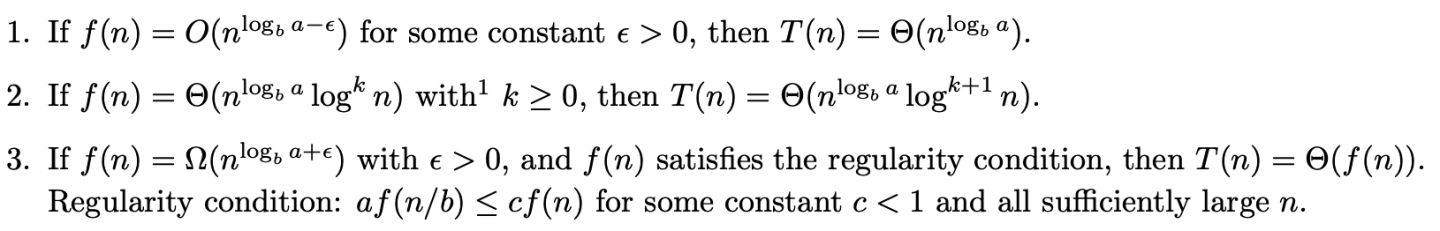
\includegraphics[scale=0.39]{src/Basic/tc-1.jpg}
			 		\end{figure}
			 		
			 \section{Ds}
			 	\subsection{链表}
			 		\inputminted{cpp}{src/Ds/List.cpp}
			 	\subsection{哈希表}
			 		\inputminted{cpp}{src/Ds/Hash_table.cpp}
			 	\subsection{并查集}
			 		\inputminted{cpp}{src/Ds/Dsu.cpp}
			 	\subsection{树状数组}
			 		\inputminted{cpp}{src/Ds/Fenwick_tree.cpp}
			 	\subsection{线段树}
			 		\inputminted{cpp}{src/Ds/Segment_tree.cpp}
			 	\subsection{轻重链剖分}
			 		\inputminted{cpp}{src/Ds/Hld.cpp}
			 	\subsection{主席树}
			 		\inputminted{cpp}{src/Ds/Persistent_seg.cpp}
			 	\subsection{李超树}
			 		\inputminted{cpp}{src/Ds/Li_chao_tree.cpp}
			 	\subsection{珂朵莉树}
			 		\inputminted{cpp}{src/Ds/Odt.cpp}
			 \section{Dp}
			 	\subsection{一些注意事项}
			 		其实动态规划的本质是,在整个状态空间中,建立了一张 DAG(有向无环图),这保证了动态规划的 \textbf{无后效性}(不会成环)。其中,每一个节点对应一个 \textbf{状态},同层的一系列节点称之为 \textbf{阶段},它对应的就是一个 \textbf{子问题}。
			 		
			 		而 \textbf{最优子结构} 则是,对于一个问题的最优解,它一定包含了子问题的最优解,或者说,一个问题的最优解应当由子问题的最优解导出,而 \textbf{决策} 则是这张图上的有向边。
			 		
			 		贪心算法其实也是满足了最优子结构的,只是它和动态规划的转移不同,它每次只 \textbf{浅显} 的取了 \textbf{当前局面} 下的最优解。
			 		
			 		动态规划则是,从先前的(多个)子问题当中,找到当前局面的最优解。
			 		
			 		换句话来说,动态规划就是,对于一些满足最优子结构性质的信息,通过分割子问题,在子问题间无后效性转移,求得最终解的算法。
			 		
			 		\begin{itemize}
			 			\item dp 数组当中应当记录两个东西,一个是阶段,一个是状态,阶段是一定要确定清楚的,状态可以先暂时不管,慢慢根据转移的需求来确定。
			 			\item 当我们发现 dp 的状态有点多,复杂度高的时候,不妨考虑精简状态,看看哪些状态是一定不可能转移的,以此达到排除冗杂状态的目的。
			 			\item 设计 dp 阶段时一定不要拘泥于基本情况,要思考更深入的情况。
			 			\item 考虑 dp 的时候,一定不要考虑以后的阶段怎么处理,我们只关心怎么分割当前的子问题,只关心怎么样覆盖完状态空间。
			 			\item 对于一类计数 dp 问题,有一个很重要的前提条件:\textbf{一种合法的基本情况和一个合法的转移序列是唯一对应的},这样,我们处理的信息天然就满足不重不漏性质,只需要保证转移合法,就能覆盖整个状态空间。
			 			\item 如果大步大步的转移比较困难,类似本题中的成段转移,不如考虑分割一下,变成小步小步的加入和新建,这样能大幅降低思考难度。
			 		\end{itemize}
		 		\subsection{背包 DP}
		 			\inputminted{cpp}{src/Dp/Pack.cpp}
			 	\subsection{数位 DP}
			 		\inputminted{python}{src/Dp/Dight_dp.py}
			 	\subsection{子集卷积/SOS DP}
			 		\inputminted{cpp}{src/Dp/Sos_dp.cpp}
			 	\subsection{斜率优化}
			 		可以斜率优化的方程通常具有以下形式:
			 		
			 		$dp(i) = \min\limits_{j = L(i)}^{R(i)}\{dp(j) + val(i, j)\}$,其中 $val(i, j)$ 为一个关于 $i, j$ 的多项式,$L(i), R(i)$ 为一个关于 $i$ 的函数,用于限制 $j$ 的范围。
			 		
			 		并且 $val(i, j)$ 存在形如 $i \times j$ 的项,与单调队列优化的仅有 $i, j$ 项不同。
			 		
			 		斜率优化的思想是,先拆掉 $L(i), R(i)$ 的限制,将所有决策点转化为二维平面上的点,将方程转化为一个一次函数来进行决策,在决策时再加上 $L(i), R(i)$ 的限制,具体来说,我们建立以下映射:
			 		
			 		- 将仅和 $j$ 相关的项看作 $y$,记这些项组成的多项式为 $y_i$,形如 $dp(j) + v(j) + \dots$。
			 		- 将和 $i,j$ 同时相关的项看作 $k,x$,其中 $i$ 这一部分作为 $k$,记为 $k_i$,$j$ 这一部分作为 $x$,记为 $x_j$,式子形如 $C_1\times(C_2 - v(i)) \times w(j)$(其中 $C_1,C_2$ 为常量),那么 $k_i = C_1\times(C_2 - v(i)), x_j = w(j)$
			 		- 将仅和 $i$ 相关的项看作 $b$,记为 $b_i$,为了方便我们把常量也算进这一部分,式子形如 $dp(i) + v(i) \times w(i) + C$,我们要最小化的就是这一部分(本质是最小化 $dp(i)$,其它的是常量所以无所谓。)
			 		
			 		(以上的式子只是做一个参考理解,需要根据实际情况来改变。)
			 		
			 		然后,问题就转化为,给定一堆平面上的点 $(x_j, y_j)$,对于一条直线 $y = k_ix + b_i$,我们需要选择一个满足 $L(i) \le j \le R(i)$ 限制的 $(x_j, y_j)$ 代入直线,使得 $b_i$ 最小。
			 		
			 		这部分的做法就是维护凸壳了。
			 		
			 		对于 $L(i), R(i)$ 的下标限制:
			 		\begin{itemize}
			 			\item 如果是类似本题的 $0 \le j < i$,说明不需要删除决策点,而且每次只会在尾部插入决策,我们枚举就好了
			 			\item 如果 $L(i), R(i)$ 是随 $i$ 单调变化的,我们就需要使用单调队列来排除冗杂
			 			\item 如果是没啥单调性的,也就是说一般要支持在任意位置插入删除决策点,就需要使用平衡树或者 CDQ 分治。
			 		\end{itemize}
			 		对于斜率的限制,只需要看斜率是否单调递增即可:
			 		\begin{itemize}
			 			\item 如果斜率随 $i$ 单调递增,那么可以直接使用单调队列取队头转移。
			 			\item 如果斜率不随 $i$ 单调递增,我们就需要在凸壳上二分答案找到最优决策点。
			 		\end{itemize}
			 		对于 $x_j$ 的限制,只需要看它是否随 $j$ 单调递增即可。
			 		\begin{itemize}
			 			\item 如果它随 $j$ 单调递增,那么我们就只需要一个一个插入决策就行。
			 			\item 如果它不随 $j$ 单调递增,那么我们就需要使用平衡树 / CDQ 分治来支持插入决策点的操作,注意 CDQ 维护的时候还要对前一半排序。
			 		\end{itemize}
			 		
			 		Last but not least: 如果使用交叉相乘来避免精度问题,要小心数据范围,如果直接使用浮点数,要记得,eps 不要开太小了,要视情况而定。
			 		
			 \section{Math}
			 	\subsection{线性求逆元以及组合数}
			 		\inputminted{cpp}{src/Math/Comb_inv.cpp}
			 	\subsection{组合数性质}
			 		二项式定理:
			 	
				 	$$
				 	(a + b)^n = \sum\limits_{i = 0}^{n}\dbinom{n}{i}a^{n - i}b^{i}
				 	$$
				 	
				 	一些组合数性质:
				 	
				 	I. 
				 	
				 	$$
				 	\dbinom{n}{m}=\dbinom{n}{n-m}
				 	$$
				 	
				 	这个是显然的,因为你选 $m$ 个和选 $n - m$ 个的情况是捆绑起来的。
				 	
				 	II.
				 	
				 	$$
				 	\dbinom{n}{k} = \dfrac{n}{k} \dbinom{n-1}{k-1}
				 	$$
				 	
				 	这个也是显然的,根据定义展开就可以得到。
				 	
				 	也可以写作
				 	
				 	$$
				 	k\dbinom{n}{k} = n\dbinom{n - 1}{k - 1}
				 	$$
				 	
				 	III.
				 	
				 	$$
				 	\dbinom{n}{m}=\dbinom{n-1}{m}+\dbinom{n-1}{m-1}
				 	$$
				 	
				 	这个就是组合数的递推式,也可以看作是杨辉三角。
				 	
				 	IV. 
				 	
				 	$$
				 	\dbinom{n}{0}+\dbinom{n}{1}+\cdots+\dbinom{n}{n}=\sum_{i=0}^n\dbinom{n}{i}=2^n
				 	$$
				 	
				 	这是二项式定理的特殊情况。取 $a=b=1$ 就可以了。
				 	
				 	
				 	V.
				 	
				 	$$
				 	\sum_{i=0}^n(-1)^i\dbinom{n}{i}=[n=0]
				 	$$
				 	
				 	二项式定理的另一种特殊情况,可取 $a=1, b=-1$。式子的特殊情况是取 $n=0$ 时答案为 $1$。
				 	
				 	后面那个是 Iverson Bracket.
				 	
				 	VI.
				 	
				 	$$
				 	\sum_{i=0}^m \dbinom{n}{i}\dbinom{m}{m-i} = \dbinom{m+n}{m}\ \ \ (n \geq m)
				 	$$
				 	
				 	这个就是范德蒙德卷积的推论。
				 	
				 	VII.
				 	
				 	$$
				 	\sum_{i=0}^n\dbinom{n}{i}^2=\dbinom{2n}{n}
				 	$$
				 	
				 	仍旧是范德蒙德卷积的推论.
				 	
				 	VIII.
				 	
				 	$$
				 	\sum_{l=0}^n\dbinom{l}{k} = \dbinom{n+1}{k+1}
				 	$$
				 	
				 	通过组合分析一一考虑 $S={a_1, a_2, \cdots, a_{n+1}}$ 的 $k+1$ 子集数可以得证,在恒等式证明中比较常用。
				 	
				 	IX.
				 	
				 	$$
				 	\dbinom{n}{r}\dbinom{r}{k} = \dbinom{n}{k}\dbinom{n-k}{r-k}
				 	$$
				 	
				 	用定义展开一下就可以证明了,式子形式很好记。
				 	
				 	X.
				 	
				 	$$
				 	\sum_{i=0}^n\dbinom{n-i}{i}=F_{n+1}
				 	$$
				 	
				 	其中 $F$ 是斐波那契数列。
			 	\subsection{范德蒙德卷积}
				 	范德蒙德卷积
				 	
				 	$$
				 	\sum\limits_{i = 0}^k \dbinom{n}{i}\dbinom{m}{k - i} = \dbinom{n + m}{k}
				 	$$
				 	
				 	也可以写成:
				 	
				 	$$
				 	\sum\limits_{i = -r}^s \dbinom{n}{r + i} \dbinom{m}{s - i} = \dbinom{n + m}{r + s}
				 	$$
			 	\subsection{快速幂}
			 		\inputminted{cpp}{src/Math/Qpow.cpp}
			 	\subsection{矩阵乘法}
			 		\inputminted{cpp}{src/Math/Matrix_mul.cpp}
			 	\subsection{高斯消元}
			 		\inputminted{cpp}{src/Math/Gauss_cut.cpp}
			 	\subsection{质数}
			 		\inputminted{cpp}{src/Math/Primes.cpp}
			 	\subsection{约数}
			 		\inputminted{cpp}{src/Math/Factors.cpp}
			 	\subsection{Exgcd}
			 		\inputminted{cpp}{src/Math/Ex_gcd.cpp}
			 	\subsection{中国剩余定理}
			 		\inputminted{cpp}{src/Math/Crt.cpp}
			 		
			 	\subsection{ExCRT}
			 		考虑两个方程怎么做。
			 		
			 		假设 $x \equiv a_1 \pmod{m_1}, x \equiv a_2 \pmod{m_2}$。
			 		
			 		按照类似 $\gcd$ 那边的套路:
			 		
			 		$x = m_1p + a_1 = m_2q + a_2, p, q \in \mathbb{Z}$。
			 		
			 		然后可以知道 $m_1p - m_2q = a_2 - a_1$,然后这东西就是类似线性同余的东西。有解当且仅当 $\gcd(m_1, m_2)\ |\ a_2 - a_1$。
			 		
			 		然后就 exgcd 解一下,显然这两个方程的解应该是 $m_2q + a_2 \pmod{\operatorname{lcm}(m_1, m_2)}$。
			 		
			 		然后我们就直接合并多个方程就可以了。
			 	\subsection{Lucas 定理}
			 		对于任意质数 $p$,存在如下定理:
			 		
			 		$$
			 		\dbinom{n}{m} \equiv \dbinom{\lfloor\frac{n}{p}\rfloor}{\lfloor\frac{m}{p}\rfloor} \cdot \dbinom{n \bmod p}{m \bmod p} \pmod p
			 		$$
			 		
			 	\subsection{Ex Lucas}
			 		
			 		考虑类似 exCRT 的经典套路,我们分解质因数,用 CRT 构造一个方程然后合并,这样每个方程里面都是一个 Lucas。
			 		
			 		也就是,令 $p = \prod\limits_{i = 1}^ra_{r}^{c_r}$。
			 		
			 		然后因为任意 $a_{i}^{c_i}, a_{j}^{c_j}$ 互质,所以我们把他们当作模数。
			 		
			 		由 CRT,令 $\dbinom{n}{m}$ 为未知数,有:
			 		
			 		$$
			 		\begin{cases}
			 			c_1 &\equiv \dbinom{n}{m} \pmod {a_{1}^{c_1}} \\
			 			c_2 &\equiv \dbinom{n}{m} \pmod {a_{2}^{c_2}} \\
			 			&\cdots\\
			 			c_r &\equiv \dbinom{n}{m} \pmod {a_{r}^{c_r}}
			 		\end{cases}
			 		$$
			 		
			 		可以由此解出未知数在模 $p$ 意义下的唯一解 $\dbinom{n}{m} \bmod p$
			 	\subsection{数论相关结论}
			 		\textbf{算术基本定理}:任何一个大于 $1$ 的正整数都可以唯一分解为有限个质数的乘积。
			 	
			 		也叫唯一分解定理,可以写成 $N = p_1^{c1}\times p_2^{c2}\times p_3^{c3}\times \dots p_m^{cm}, c_i \in \mathbb{N}^*, p_i < p_{i + 1},\text{PRIME}(p_i)$。
			 	
			 		\textbf{唯一分解定理的三个推论}:
			 		
			 		1. 若 $n \in \mathbb{N}^*$,则 $n$ 的正约数集合为 $\{x | x = p_1^{b_1}p_2^{b_2}\dots p_m^{b_m},b_i \le 	c_i\}$。
			 		2. $n$ 的正约数个数为 $\prod\limits_{i = 1}^m(c_i+ 1)$
			 		3. $n$ 的正约数之和为 $(1+p_1+p_1^2+p_1^3+\dots +p_1^{c_1})\times\dots(1+p_m+p_m^2+p_m^3+\dots +p_m^{c_m}) = \prod\limits_{i = 1}^m(\sum\limits_{j = 1}^{c_i} p_i^{j})$
			 	
				 	\textbf{约数个数和结论}:$1\sim n$ 所有数的约数个数之和约为 $n\log n$ 个
				 	
				 	\textbf{更相减损术}:
				 	\begin{itemize}
				 		\item $\forall a,b \in \mathbb{N},a\ge b$ 有 $\gcd(a,b) = \gcd(b, a-b) = \gcd(a, a-b)$
				 		\item $\forall a,b \in \mathbb{N}$,有 $\gcd(2a,2b) = 2\gcd(a,b)$。
				 	\end{itemize}
			 	
				 	\textbf{欧拉函数的性质}
				 	
				 	性质1:$\forall n > 1, 1\sim n$ 中与 $n$ 互质的数的和为 $n\cdot\varphi(n)/2$。
				 	
				 	由更相减损术,和 $n$ 互质的数必然成对出现,且均值为 $n/2$,证毕。
				 	
				 	性质2:欧拉函数为积性函数,且有:$\gcd(a,b)=1\Rightarrow \varphi(ab)=\varphi(a)\cdot\varphi(b)$。
				 	
				 	展开计算式就行了。
				 	
				 	性质3:(积性函数的性质):在唯一分解定理背景下,若 $f$ 为积性函数,则有:$f(n)=\prod\limits_{i=1}^mf(p_i^{c_i})$
				 	
				 	显然任意的 $p_i^{c_i}$ 和 $p_j^{c_j}$ 必然互质,由积性函数的性质,对整体应用结论,可以得到原式。
				 	
				 	性质4:若 $p$ 为质数,若 $p|n$ 且 $p^2\not|n$,则 $\varphi(n)=\varphi(n/p)\varphi(p)=\varphi(n/p)\cdot(p-1)$。
				 	
				 	积性函数的性质,显然,常用于递推。
				 	
				 	性质5:若 $p$ 为质数,若 $p|n$ 且 $p^2|n$,则 $\varphi(n)= \varphi(n/p)\times p$
				 	
				 	因为 $n/p$ 和 $p$ 不互质,所以只能展开计算式得到,常用于递推。
				 	
				 	性质6:$\sum_{d|n}\varphi(d)=n$。
				 	
				 	很有意思的性质,先对 $n$ 分解质因数,令 $f(x)=\sum_{d|x}\varphi(d)$。
				 	
				 	显然 $f(p_i^{c_i}) = \varphi(1)+\varphi(p_i)+\varphi(p_i^{2})+\dots+\varphi(p_i^{c_i}) = p_i^{c_i}$(由性质 $5$ 可以发现是一个等比数列求和)。
				 	
				 	然后发现若 $\gcd(n,m)=1$,$f(nm)=(\sum_{d|n}\varphi(d))\cdot(\sum_{d|m}\varphi(d))=f(n)f(m)$。
				 	
				 	所以 $f$ 是积性函数,由积性函数性质可以得到原式成立。
				 	
				 	结论 1:对于足够大的 $n \in \mathbb{N}^*$,$[1,n]$ 中的素数个数约为 $\frac{n}{\ln n}$ 个 (**对数结论**)
				 	
				 	结论 2:若 $\lnot \text{PRIME}(n)$,则 $\exists T \in [2,\sqrt{n}]$,使得 $T|n$。(**根号结论**)
			 	\subsection{容斥原理}
			 		若有 $n$ 个集合 $S_1 \dots S_n$,并且集合之间可能有交集。
			 	
				 	那么 $|\bigcup S_i|$ 就等于 $\sum_i |S_i| - \sum_{i, j} |S_i \cap S_j| + \sum_{i, j, k} |S_i \cap S_j \cap S_k| \dots + (-1)^{n + 1} \sum_{a_1, \dots a_n} |\bigcap_j S_{a_j}|$。
				 	
				 	$a_1, \dots a_n$ 是用来枚举集合的。
				 	
				 	这个柿子也可以简述为,多个集合的并集大小等于奇数个集合的交集的大小之和减去偶数个集合的交集大小之和。
				 	
				 	或者描述为:
				 	
				 	$\sum$ 在任意一个集合内的元素个数总和 $−\sum$ 在任意两个集合交内的元素个数总和 $+\sum$ 在任意三个集合交内的元素个数总和...
				 	
				 	注意这里“在任意两个集合交集内的元素个数总和”是要算重的,也就是说如果 $x$ 在 $A\cap B \cap C$ 当中,那么在算任意两个集合交内的元素个数总和时,$x$ 的贡献就是 $3$。
				 	
				 	这么做其实就是为了方便计数,因为有多个条件但是只是“至少”满足一个或者几个的时候,无法比较方便的知道哪些条件满足,哪些条件不满足。
				 	
				 	所以我们直接只考虑某些特定的条件一定被满足的时候方案数,其它的直接不管怎么搞,反正不合法或者重复的肯定会被容斥掉。
				 	
				 	这就是一种“至少转强制”的思想。
			 	\subsection{二项式反演}
			 	 	用于解决“某个物品恰好若干个” 的一类问题。
			 	 	
			 		设 $g(n)$ 表示至多 $n$ 种的方案数,$f(n)$ 表示恰好 $n$ 种的方案数,则有
			 		
			 		$$
			 		g(n) =  \sum\limits_{i = 0}^n \dbinom{n}{i} f(i) \iff f(n) = \sum\limits_{i = 0}^n (-1)^{n - i}\dbinom{n}{i}g(i)
			 		$$ 
			 		
			 		设 $g(n)$ 表示至少 $n$ 种的方案数,$f(n)$ 表示恰好 $n$ 种的方案数,则有
			 		
			 		$$
			 		g(n) = \sum\limits_{i = k}^n\dbinom{i}{k}f(i) \iff f(k) = \sum\limits_{i = k}^n (-1)^{i - k}\dbinom{i}{k} g(i)
			 		$$
			 	
			 \section{Graph}
			 	\subsection{SPFA 以及负环}
			 		\inputminted{cpp}{src/Graph/Spfa.cpp}
			 	\subsection{Dijkstra}
			 		\inputminted{cpp}{src/Graph/Dijkstra.cpp}
			 	\subsection{Floyd 以及最小环}
			 		\inputminted{cpp}{src/Graph/Floyd.cpp}
			 	\subsection{Kruskal}
			 		\inputminted{cpp}{src/Graph/Kruskal.cpp}
			 	\subparagraph{Prim}
			 		\inputminted{cpp}{src/Graph/Prim.cpp}
			 	\subsection{倍增 LCA}
			 		\inputminted{cpp}{src/Graph/Multiper_lca.cpp}
			 	\subsection{Tarjan LCA}
			 		\inputminted{cpp}{src/Graph/Tarjan_Lca.cpp}
			 	\subsection{拓扑排序}
			 		\inputminted{cpp}{src/Graph/Topo_sort.cpp}
			 	\subsection{欧拉回路}
			 		\inputminted{cpp}{src/Graph/Euler_path.cpp}
			 	\subsection{强连通分量}
			 		\inputminted{cpp}{src/Graph/Tarjan_scc.cpp}
			 	\subsection{边双连通分量}
			 		\inputminted{cpp}{src/Graph/Tarjan_edcc.cpp}
			 	\subsection{点双连通分量}
			 		\inputminted{cpp}{src/Graph/Tarjan_vdcc.cpp}
			 	\subsection{虚树}
			 		\inputminted{cpp}{src/Graph/Virtual_tree.cpp}
			 \section{String}
			 	\subsection{Kmp}
			 		\inputminted{cpp}{src/String/Kmp.cpp}
			 	\subsection{Trie}
			 		\inputminted{cpp}{src/String/Trie.cpp}
			 	\subsection{01Trie}
			 		\inputminted{cpp}{src/String/01_trie.cpp}
			 	\subsection{Ac Automaton}
			 		\inputminted{cpp}{src/String/Ac_automaton.cpp}
			 \section{Misc}
			 	\subsection{莫队}
			 		\inputminted{cpp}{src/Misc/Mo.cpp}
		\end{spacing}
			\endgroup
	\end{multicols}
	
	\begin{center}
		\LARGE{Good Luck \&\& Have Fun!}
	\end{center}
		
	\end{document}
	%THE SCL ENDS
